% !TeX program = lualatex
\documentclass[10pt,a4paper]{article}

\usepackage{fontspec}
\defaultfontfeatures{Ligatures=TeX}
% Font sans moderno coerente col documento Criteri CISF27 (Liberation Sans con fallback Arial su macOS)
\IfFontExistsTF{Liberation Sans}{
  \setsansfont{Liberation Sans}[
    BoldFont={Liberation Sans Bold},
    ItalicFont={Liberation Sans Italic},
    BoldItalicFont={Liberation Sans Bold Italic}
  ]
  \setmainfont{Liberation Sans}
}{
  \setsansfont{Arial}[
    BoldFont={Arial Bold},
    ItalicFont={Arial Italic},
    BoldItalicFont={Arial Bold Italic}
  ]
  \setmainfont{Arial}
}
\setmonofont{Latin Modern Mono}

\usepackage[italian]{babel}
\usepackage[margin=1.7cm,top=1.75cm,bottom=1.75cm,footskip=0.9cm,headheight=0.95cm]{geometry}
\linespread{0.97}
\usepackage{xcolor}
\usepackage{graphicx}
\usepackage{tabularx,booktabs,colortbl}
\usepackage{titlesec}
\usepackage{fancyhdr}
\usepackage{enumitem}
\usepackage{tikz}
\usepackage{microtype}
\usepackage{fontawesome5}
\usepackage[most]{tcolorbox}
\usepackage{lastpage}
\usepackage[colorlinks=true,linkcolor=cisfBurgundy,urlcolor=cisfBurgundy,pdfencoding=auto]{hyperref}

\hypersetup{
  pdftitle={Codice Etico Ufficiale — CISF27 Bologna},
  pdfauthor={Comitato Organizzatore CISF27 — AISF Comitato Locale di Bologna},
  pdfsubject={Principi etici, Safe Space, sponsorizzazioni etiche, sostenibilita Plastic-freER, apartiticita e trasparenza — XI Conferenza Italiana Studenti di Fisica}
}

% =========================================================================
% PALETTE COLORI UFFICIALE CISF27 BOLOGNA
% =========================================================================
\definecolor{cisfBurgundy}{HTML}{7A0019}     % Rosso Cardinale / Bologna
\definecolor{cisfBurgundyDark}{HTML}{500010} % Rosso Scuro Istituzionale
\definecolor{cisfRed}{HTML}{9E2A2B}          % Rosso Terracotta
\definecolor{cisfGold}{HTML}{D97706}         % Oro / Amber Portici
\definecolor{cisfAmber}{HTML}{F59E0B}        % Amber Chiaro
\definecolor{cisfGreen}{HTML}{15803D}        % Verde Sostenibilita #Plastic-freER
\definecolor{cisfNavy}{HTML}{1E293B}         % Slate 800
\definecolor{cisfGray}{HTML}{FAF7F2}         % Sfondo Caldo Card (Avorio Bologna)
\definecolor{cisfSlateBg}{HTML}{F8FAFC}      % Sfondo Neutro Card
\definecolor{cisfBorder}{HTML}{E2E8F0}       % Bordo Card
\definecolor{cisfMuted}{HTML}{64748B}        % Testo Secondario

% =========================================================================
% STILE INTESTAZIONI E PARAGRAFI
% =========================================================================
\setlength{\parindent}{0pt}
\setlength{\parskip}{0.26em}

\titleformat{\section}
  {\large\bfseries\color{cisfBurgundy}}{Art.\,\thesection\ ---\ }{0pt}{}[\vspace{2pt}{\color{cisfBurgundy!35}\titlerule[0.8pt]}]
\titleformat{\subsection}
  {\normalsize\bfseries\color{cisfBurgundyDark}}{\thesubsection}{0.6em}{}

\titlespacing*{\section}{0pt}{8pt}{4pt}
\titlespacing*{\subsection}{0pt}{6pt}{2pt}

\setlist[itemize]{
  label=\textcolor{cisfBurgundy}{\scriptsize\faChevronRight},
  leftmargin=1.35em,
  itemsep=0.12em,
  topsep=0.15em
}

% =========================================================================
% HEADER & FOOTER
% =========================================================================
\pagestyle{fancy}
\fancyhf{}
\fancyhead[L]{\small\color{cisfMuted}\textbf{CISF27 Bologna} --- Codice Etico Ufficiale}
\fancyhead[R]{\small\color{cisfBurgundy}\textbf{AISF | Comitato Locale di Bologna}}
\fancyfoot[L]{\footnotesize\color{cisfMuted}Conferenza Italiana Studenti di Fisica (19--23 aprile 2027) $\cdot$ \href{https://ai-sf.it/cisf27/criteri}{ai-sf.it/cisf27/criteri}}
\fancyfoot[R]{\footnotesize\color{cisfBurgundy}\textbf{Pag.\,\thepage/\pageref*{LastPage}}}
\renewcommand{\headrulewidth}{0.4pt}
\renewcommand{\footrulewidth}{0.4pt}
\renewcommand{\headrule}{\hbox to\headwidth{\color{cisfBurgundy!35}\leaders\hrule height \headrulewidth\hfill}}
\renewcommand{\footrule}{\hbox to\headwidth{\color{cisfBurgundy!35}\leaders\hrule height \footrulewidth\hfill}}

\fancypagestyle{firstpage}{
  \fancyhf{}
  \fancyfoot[L]{\footnotesize\color{cisfMuted}Conferenza Italiana Studenti di Fisica (19--23 aprile 2027) $\cdot$ \href{https://ai-sf.it/cisf27/criteri}{ai-sf.it/cisf27/criteri}}
  \fancyfoot[R]{\footnotesize\color{cisfBurgundy}\textbf{Pag.\,\thepage/\pageref*{LastPage}}}
  \renewcommand{\headrulewidth}{0pt}
  \renewcommand{\footrulewidth}{0.4pt}
  \renewcommand{\headrule}{}
  \renewcommand{\footrule}{\hbox to\headwidth{\color{cisfBurgundy!35}\leaders\hrule height \footrulewidth\hfill}}
}

% =========================================================================
% BOX MODERNI CON TCOLORBOX
% =========================================================================
\newtcolorbox{cisfcallout}[2][]{
  enhanced,
  breakable,
  colback=cisfGray,
  colframe=cisfBurgundy,
  arc=2.5mm,
  boxrule=0.9pt,
  leftrule=3.5mm,
  top=8pt,bottom=7pt,left=10pt,right=10pt,
  title=\textbf{#2},
  coltitle=white,
  attach boxed title to top left={yshift=-2.2mm,xshift=4mm},
  boxed title style={colback=cisfBurgundy,arc=1.5mm,boxrule=0pt,top=2pt,bottom=2pt,left=6pt,right=6pt},
  fonttitle=\small\sffamily,
  fontupper=\small\sffamily,
  before skip=8pt,
  after skip=8pt,
  #1
}

\newtcolorbox{cisfalert}[2][]{
  enhanced,
  breakable,
  colback=cisfGold!9!white,
  colframe=cisfGold,
  arc=2.5mm,
  boxrule=0.9pt,
  leftrule=3.5mm,
  top=8pt,bottom=7pt,left=10pt,right=10pt,
  title=\textbf{#2},
  coltitle=white,
  attach boxed title to top left={yshift=-2.2mm,xshift=4mm},
  boxed title style={colback=cisfGold,arc=1.5mm,boxrule=0pt,top=2pt,bottom=2pt,left=6pt,right=6pt},
  fonttitle=\small\sffamily,
  fontupper=\small\sffamily,
  before skip=8pt,
  after skip=8pt,
  #1
}

\newtcolorbox{cisfgreen}[2][]{
  enhanced,
  breakable,
  colback=cisfGreen!6!white,
  colframe=cisfGreen,
  arc=2.5mm,
  boxrule=0.9pt,
  leftrule=3.5mm,
  top=8pt,bottom=7pt,left=10pt,right=10pt,
  title=\textbf{#2},
  coltitle=white,
  attach boxed title to top left={yshift=-2.2mm,xshift=4mm},
  boxed title style={colback=cisfGreen,arc=1.5mm,boxrule=0pt,top=2pt,bottom=2pt,left=6pt,right=6pt},
  fonttitle=\small\sffamily,
  fontupper=\small\sffamily,
  before skip=8pt,
  after skip=8pt,
  #1
}

\newtcolorbox{cisfcontact}[2][]{
  enhanced,
  colback=cisfSlateBg,
  colframe=cisfBurgundyDark,
  arc=3mm,
  boxrule=1pt,
  leftrule=4mm,
  top=7pt,bottom=7pt,left=11pt,right=11pt,
  title=\textbf{#2},
  coltitle=white,
  attach boxed title to top left={yshift=-2.2mm,xshift=4mm},
  boxed title style={colback=cisfBurgundyDark,arc=1.5mm,boxrule=0pt,top=2pt,bottom=2pt,left=7pt,right=7pt},
  fonttitle=\small\sffamily,
  fontupper=\small\sffamily,
  before skip=6pt,
  after skip=6pt,
  #1
}

\begin{document}
\thispagestyle{firstpage}
\color{cisfNavy}

% =========================================================================
% TESTATA CON LOGHI E BANNER BOLOGNA
% =========================================================================
\begin{center}
  \begin{minipage}[c]{0.27\textwidth}
    \centering
    
\includegraphics[height=1.25cm]{logos/aisf.png}
  \end{minipage}\hfill
  \begin{minipage}[c]{0.42\textwidth}
    \centering
    
\includegraphics[height=1.55cm]{logos/cisf27.png}
  \end{minipage}\hfill
  \begin{minipage}[c]{0.27\textwidth}
    \centering
    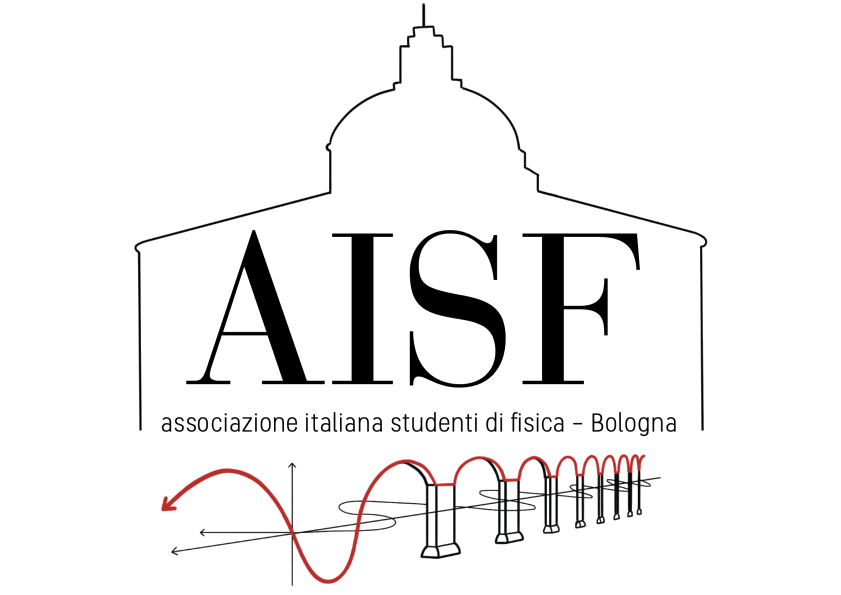
\includegraphics[height=1.35cm]{logos/aisf-bolo.png}
  \end{minipage}
\end{center}

\vspace{0.2cm}

\begin{tcolorbox}[
  enhanced,
  colback=cisfBurgundy,
  colframe=cisfBurgundyDark,
  arc=3.5mm,
  boxrule=1.2pt,
  top=11pt,bottom=11pt,left=15pt,right=15pt
]
  \begin{minipage}[c]{0.70\textwidth}
    {\color{cisfAmber}\footnotesize\textbf{AISF --- COMITATO LOCALE DI BOLOGNA}}\\[3pt]
    {\color{white}\LARGE\textbf{Codice Etico di CISF27 Bologna}}\\[3pt]
    {\color{white!90}\normalsize XI Conferenza Italiana Studenti di Fisica --- \textit{Le Traiettorie della Fisica}}\\[4pt]
    {\color{cisfAmber!85}\footnotesize Documento Ufficiale del Comitato Organizzatore $\cdot$ Valido per l'intera Conferenza}
  \end{minipage}
  \hfill
  \begin{minipage}[c]{0.27\textwidth}
    \begin{flushright}
      \color{white}\footnotesize
      \textbf{Date:} 19--23 aprile 2027\\
      \textbf{Sede:} Bologna (BO)\\
      \textbf{Stato:} Documento Pubblico\\
      \textbf{Email:} \href{mailto:cisf27@ai-sf.it}{\color{white}cisf27@ai-sf.it}
    \end{flushright}
  \end{minipage}
\end{tcolorbox}

\vspace{0.2cm}

% =========================================================================
% PREAMBOLO
% =========================================================================
\begin{cisfcallout}{\faBalanceScale\hspace{0.5em}Preambolo e Ambito di Applicazione}
La \textbf{Conferenza Italiana Studenti di Fisica 2027 (CISF27)}, promossa dall'Associazione Italiana Studenti di Fisica (\textbf{AISF}, A.P.S. no-profit e Comitato Territoriale Italiano dell'\textit{International Association of Physics Students} -- \textbf{IAPS}) e organizzata dal Comitato Locale di Bologna, si fonda sulla convinzione che la comunità scientifica debba essere un luogo libero, equo, accogliente, sostenibile e trasparente.

Il presente \textbf{Codice Etico}, adottato dal Comitato Organizzatore (CO) di CISF27 in coerenza con lo \textbf{Statuto di AISF} (artt.\,2, 14, 16 e 17), il \textbf{Piano Strategico AISF} e il \textbf{\textit{Code of Conduct} di IAPS}, definisce i principi vincolanti che regolano la Conferenza in tutte le sue fasi: dalla presentazione delle candidature fino allo svolgimento di sessioni scientifiche, visite ai laboratori, momenti conviviali, Assemblea Generale Annuale (AGA), nonché tutte le comunicazioni sui canali digitali e le relazioni con enti, sponsor e fornitori.

\textbf{Destinatari:} il presente Codice si applica senza eccezione a tutte le persone candidate e partecipanti, ai membri del Comitato Organizzatore e del Comitato Esecutivo AISF, agli ausiliari e volontari, a relatori, ospiti, patrocinatori, sponsor e fornitori coinvolti in CISF27.
\end{cisfcallout}

% =========================================================================
% ART. 1: INCLUSIVITA, PARITA E ACCESSIBILITA
% =========================================================================
\section{Inclusività, Parità di Genere e Accessibilità}

In conformità con l'Art.\,14 dello Statuto AISF e con i principi ispiratori dell'Associazione, CISF27 opera senza alcuna discriminazione e si impegna ad abbattere barriere sociali, economiche, accademiche, fisiche e relazionali: \emph{«la CISF è di tutti»}.

\begin{itemize}
  \item \textbf{Parità di genere e tutela delle identità:} il CO si impegna attivamente a raggiungere la \textbf{parità di genere} tra le persone partecipanti, tutelando pienamente ogni identità ed espressione di genere, anche attraverso l'utilizzo di un linguaggio rispettoso, il riguardo dei pronomi scelti e un'assegnazione attenta e concordata delle camere presso il \textit{Combo Bologna}.
  \item \textbf{Accessibilità fisica, logistica e alimentare:} in fase di candidatura e prima dell'evento vengono raccolte, in forma strettamente riservata, le indicazioni relative a disabilità, necessità fisiche, logistiche, psicologiche, allergie, intolleranze e regimi alimentari. \textbf{In nessun modo tali segnalazioni influiscono sulla selezione}, ma servono esclusivamente a consentire al CO di rendere l'evento realmente accessibile e sereno per ogni persona.
  \item \textbf{Accessibilità economica e spirito no-profit:} CISF27 è una conferenza studentesca interamente \textbf{no-profit}. Il sostegno di enti pubblici, istituti di ricerca e partner etici è destinato a calmierare le quote di partecipazione e di alloggio affinché le condizioni economiche non rappresentino un ostacolo alla partecipazione. L'evento \textbf{non è a scopo di lucro.}
\end{itemize}

\clearpage

% =========================================================================
% ART. 2: SAFE SPACE E TOLLERANZA ZERO
% =========================================================================
\section{Safe Space e Tolleranza Zero verso Discriminazioni e Molestie}

Ogni persona che prende parte a CISF27 ha il diritto inviolabile di vivere un ambiente sicuro, rispettoso e privo di ostilità (\textbf{\textit{Safe Space}}), sia nei momenti accademici sia negli eventi sociali e serali.

\begin{itemize}
  \item \textbf{Divieto assoluto di discriminazione:} è vietata qualsiasi forma di discriminazione, esclusione o trattamento deteriore basato su genere, identità o espressione di genere, orientamento sessuale, origine etnica o nazionale, religione o credo, opinione politica, età, disabilità, aspetto fisico, condizione socio-economica o percorso di studi.
  \item \textbf{Tolleranza zero verso molestie e messaggi d'odio:} sono severamente proibiti molestie verbali, fisiche o sessuali, approcci indesiderati, intimidazioni, minacce, insulti, ingiurie, messaggi d'odio e qualsiasi comportamento che generi un ambiente ostile o lesivo della dignità altrui. La presenza di contenuti d'odio, minacce o affermazioni contrarie al presente Codice nella domanda di candidatura comporta il \textbf{rigetto automatico e irrevocabile della candidatura}.
  \item \textbf{Centralità del consenso:} in coerenza con il \textit{Code of Conduct} IAPS, ogni interazione personale deve basarsi sul \textbf{consenso libero, attivo, informato, esplicito e revocabile} in qualsiasi momento. Il silenzio non equivale mai a consenso, né esiste consenso valido in presenza di coercizione, pressione o alterazione psicofisica.
\end{itemize}

% =========================================================================
% ART. 3: SPONSORIZZAZIONI ETICHE E NO INDUSTRIA BELLICA
% =========================================================================
\section{Sponsorizzazioni Etiche e Rifiuto dell'Industria Bellica}

Il Comitato Organizzatore di CISF27 ha formalmente deliberato all'unanimità una linea etica chiara e trasparente per la selezione di sponsor, partner tecnici, collaborazioni e fornitori, a tutela dell'integrità morale e scientifica della Conferenza.

\begin{cisfalert}{\faIcon{shield-alt}\hspace{0.5em}Delibera Etica del CO: Rifiuto di Fondi dall'Industria Bellica e dalle Armi}
\begin{itemize}[topsep=2pt,itemsep=0.25em]
  \item \textbf{Esclusione categorica (affiliazioni dirette / di primo grado):} il CO CISF27 \textbf{rifiuta categoricamente qualsiasi finanziamento, sponsorizzazione economica o tecnica, partnership o collaborazione diretta} con aziende, gruppi industriali o enti operanti nell'\textbf{industria bellica}, nella produzione o commercializzazione di \textbf{armi} o direttamente implicati in \textbf{conflitti armati}.
  \item \textbf{Valutazione responsabile sulle relazioni indirette:} ferma restando l'esclusione inderogabile di ogni soggetto direttamente attivo nel comparto bellico o militare, eventuali relazioni finanziarie indirette (``di secondo grado'') vengono valutate collegialmente dal CO con approccio pragmatico, documentato e coerente con i principi associativi, escludendo in ogni caso qualsiasi attività di promozione militare o bellica.
  \item \textbf{Indipendenza scientifica e culturale:} nessuna sponsorizzazione o collaborazione tecnica può condizionare l'identità associativa AISF, la libertà accademica, il programma scientifico, i contenuti dei relatori o le decisioni di selezione dei partecipanti. Analoga attenzione valoriale guida la scelta delle strutture ospitanti e dei fornitori dell'evento.
\end{itemize}
\end{cisfalert}

% =========================================================================
% ART. 4: SOSTENIBILITA AMBIENTALE #PLASTIC-FREER
% =========================================================================
\section{Sostenibilità Ambientale e Adesione a \#Plastic-freER}

In piena armonia con il patrocinio concesso dalla \textbf{Regione Emilia-Romagna} (rif.\,prot.\,PG/2026/491726) e con il pilastro programmatico \textit{Energia} del tema \emph{«Le Traiettorie della Fisica»}, CISF27 adotta pratiche concrete per minimizzare la propria impronta ambientale.

\begin{cisfgreen}{\faLeaf\hspace{0.5em}Impegno Ufficiale \#Plastic-freER --- Strategia Regionale Emilia-Romagna}
\begin{minipage}[c]{0.76\linewidth}
  \begin{itemize}[label=\textcolor{cisfGreen}{\scriptsize\faCheckCircle},leftmargin=1.35em,itemsep=0.25em,topsep=1pt]
    \item \textbf{Stop alla plastica monouso:} adesione ai requisiti della strategia regionale \textbf{\#Plastic-freER}, eliminando bicchieri, stoviglie e bottiglie in plastica monouso durante coffee break, pranzi, cene sociali ed eventi della Conferenza.
    \item \textbf{Riuso e riduzione degli sprechi:} promozione di borracce riutilizzabili, materiali compostabili o riciclabili, riduzione dei materiali cartacei superflui e attenzione alla prevenzione dello spreco alimentare.
    \item \textbf{Mobilità sostenibile:} incentivazione del trasporto pubblico locale tramite la fornitura ai partecipanti di titoli di viaggio \textbf{TPER} per gli spostamenti urbani a Bologna e valorizzazione di percorsi pedonali e soluzioni di mobilità dolce.
  \end{itemize}
\end{minipage}\hfill
\begin{minipage}[c]{0.21\linewidth}
  \centering
  
\includegraphics[width=0.95\linewidth]{logos/plasticfreer.png}
\end{minipage}
\end{cisfgreen}

\clearpage

% =========================================================================
% ART. 5: APARTITICITA E NEUTRALITA ISTITUZIONALE
% =========================================================================
\section{Apartiticità, Aconfessionalità e Neutralità Istituzionale}

Coerentemente con lo Statuto di AISF, con il Piano Strategico AISF e con le delibere del CO, AISF e CISF27 sono rigorosamente \textbf{apartitiche e aconfessionali}, indipendenti da qualsiasi partito, movimento politico o gruppo di pressione.

\begin{itemize}
  \item \textbf{Indipendenza da affiliazioni politiche:} il CO rifiuta finanziamenti, patrocini di parte o affiliazioni politiche dirette, preservando la Conferenza come spazio libero, pluralista e neutrale aperto a tutta la comunità studentesca.
  \item \textbf{Divieto di propaganda:} è vietata qualsiasi forma di propaganda politica, partitica o ideologica sia nei materiali di candidatura (causa di rigetto automatico) sia negli spazi fisici, negli interventi e nei canali di comunicazione ufficiali di CISF27.
  \item \textbf{Dialogo scientifico aperto:} la neutralità partitica garantisce e protegge il confronto libero, critico e costruttivo su scienza, società, energia e futuro professionale, nel rispetto della Costituzione e dei valori democratici.
\end{itemize}

% =========================================================================
% ART. 6: TRASPARENZA, INTEGRITA E GOVERNANCE
% =========================================================================
\section{Trasparenza, Integrità e Governance Democratica}

La fiducia della comunità studentesca si fonda sulla chiarezza delle regole e sulla correttezza di ogni procedura gestionale, selettiva e finanziaria.

\begin{itemize}
  \item \textbf{Accesso pubblico ai documenti ufficiali:} sia i \textit{Criteri di Selezione Ufficiali} sia il presente \textit{Codice Etico} sono pubblicati e scaricabili liberamente sul sito ufficiale della Conferenza (\href{https://ai-sf.it/cisf27/criteri}{ai-sf.it/cisf27/criteri}), anche al di fuori del modulo di candidatura.
  \item \textbf{Supervisione del Comitato Esecutivo (EC):} ogni fase della selezione dei partecipanti è supervisionata dal Comitato Esecutivo di AISF. Ogni persona interessata può richiedere chiarimenti al CO e a EC.
  \item \textbf{Integrità e autenticità:} CISF27 promuove l'onestà intellettuale e personale. Dichiarazioni false o mendaci e motivazioni redatte con chiaro ed evidente utilizzo passivo di Intelligenza Artificiale comportano il rigetto irrevocabile della candidatura. Tutte le risorse raccolte sono gestite secondo i principi di verità, trasparenza e correttezza previsti dagli artt.\,6 e 12 dello Statuto AISF.
\end{itemize}

% =========================================================================
% ART. 7: SEGNALAZIONI, ASCOLTO RISERVATO E PROVVEDIMENTI
% =========================================================================
\section{Segnalazioni, Canali Riservati e Procedura di Intervento}

Chiunque subisca, osservi o venga a conoscenza di una violazione del presente Codice Etico --- durante la fase di candidatura, nel corso della Conferenza o nei canali digitali collegati --- può segnalarlo tempestivamente in piena riservatezza.

\begin{cisfcontact}{\faLock\hspace{0.5em}Canali Riservati dei Coordinatori Generali CISF27}
Per segnalazioni confidenziali, richieste di supporto o situazioni che compromettano il benessere e la sicurezza di una o più persone, è possibile scrivere in via riservata ai \textbf{Coordinatori Generali di CISF27}:

\vspace{0.12cm}
\renewcommand{\arraystretch}{1.15}
\begin{tabularx}{\linewidth}{@{} X X @{}}
  \textbf{\color{cisfBurgundy}Francesco Isgrò} & \textbf{\color{cisfBurgundy}Alessandro D'Agostino} \\
  \textit{Coordinatore Generale CISF27} & \textit{Coordinatore Generale CISF27} \\
  \faEnvelope\hspace{0.4em}\href{mailto:francesco.isgro@ai-sf.it}{\texttt{francesco.isgro@ai-sf.it}} &
  \faEnvelope\hspace{0.4em}\href{mailto:alessandro.dagostino@ai-sf.it}{\texttt{alessandro.dagostino@ai-sf.it}} \\
\end{tabularx}
\vspace{0.12cm}

{\footnotesize\color{cisfMuted}
\faInfoCircle\hspace{0.35em}Per richieste di informazioni generali sui criteri di selezione o sull'evento: \href{mailto:cisf27@ai-sf.it}{\texttt{cisf27@ai-sf.it}}. In caso di potenziale conflitto di interesse che coinvolga membri del Comitato Organizzatore, la segnalazione può essere rivolta direttamente al \textbf{Comitato Esecutivo (EC) di AISF} o al Collegio dei Probiviri.}
\end{cisfcontact}

\begin{itemize}
  \item \textbf{Riservatezza e protezione da ritorsioni:} ogni segnalazione è trattata con la massima riservatezza e nel pieno rispetto della persona segnalante. È assolutamente vietata ogni forma di ritorsione o intimidazione verso chi segnala o collabora all'accertamento in buona fede.
  \item \textbf{Misure cautelari e interventi immediati:} per tutelare la sicurezza dei partecipanti durante la Conferenza, i Coordinatori Generali e il CO (in raccordo con EC) possono disporre misure immediate e proporzionate --- tra cui la riassegnazione dell'alloggio, richiami formali o l'allontanamento immediato dalle attività della Conferenza senza diritto ad alcun rimborso.
  \item \textbf{Raccordo con lo Statuto AISF:} per gli associati AISF, le violazioni gravi o reiterate vengono inoltre deferite al Comitato Esecutivo ai sensi dell'\textbf{Art.\,17 dello Statuto di AISF}, che prevede (nel rispetto del contraddittorio e del diritto di ricorso al Collegio dei Probiviri) richiamo scritto, sospensione temporanea fino a un anno o esclusione definitiva dall'Associazione, ferma restando la facoltà di segnalazione alle autorità competenti in caso di illeciti di legge.
\end{itemize}

\vspace{0.05cm}
\hrule height 0.4pt
\vspace{0.15cm}

% =========================================================================
% FIRMA E CHIUSURA UFFICIALE
% =========================================================================
\noindent
\begin{minipage}[b]{0.48\textwidth}
  \footnotesize\color{cisfMuted}
  \textbf{Documento adottato dal CO CISF27 Bologna}\\
  Con il coordinamento e la supervisione del\\
  Comitato Esecutivo di AISF.\\[0.25em]
  Sito ufficiale: \href{https://ai-sf.it/cisf27/criteri}{https://ai-sf.it/cisf27/criteri}
\end{minipage}
\hfill
\begin{minipage}[b]{0.48\textwidth}
  \begin{flushright}
    \small
    \textbf{Francesco Isgrò} -- \textit{Coordinatore Generale CISF27}\\
    \textbf{Alessandro D'Agostino} -- \textit{Coordinatore Generale CISF27}\\
    \textit{e tutto il Comitato Organizzatore CISF27}
  \end{flushright}
\end{minipage}

\end{document}
